
%% bare_conf.tex
%% V1.4b
%% 2015/08/26
%% by Michael Shell
%% See:
%% http://www.michaelshell.org/
%% for current contact information.
%%
%% This is a skeleton file demonstrating the use of IEEEtran.cls
%% (requires IEEEtran.cls version 1.8b or later) with an IEEE
%% conference paper.
%%
%% Support sites:
%% http://www.michaelshell.org/tex/ieeetran/
%% http://www.ctan.org/pkg/ieeetran
%% and
%% http://www.ieee.org/

%%*************************************************************************
%% Legal Notice:
%% This code is offered as-is without any warranty either expressed or
%% implied; without even the implied warranty of MERCHANTABILITY or
%% FITNESS FOR A PARTICULAR PURPOSE! 
%% User assumes all risk.
%% In no event shall the IEEE or any contributor to this code be liable for
%% any damages or losses, including, but not limited to, incidental,
%% consequential, or any other damages, resulting from the use or misuse
%% of any information contained here.
%%
%% All comments are the opinions of their respective authors and are not
%% necessarily endorsed by the IEEE.
%%
%% This work is distributed under the LaTeX Project Public License (LPPL)
%% ( http://www.latex-project.org/ ) version 1.3, and may be freely used,
%% distributed and modified. A copy of the LPPL, version 1.3, is included
%% in the base LaTeX documentation of all distributions of LaTeX released
%% 2003/12/01 or later.
%% Retain all contribution notices and credits.
%% ** Modified files should be clearly indicated as such, including  **
%% ** renaming them and changing author support contact information. **
%%*************************************************************************
% *** Authors should verify (and, if needed, correct) their LaTeX system  ***
% *** with the testflow diagnostic prior to trusting their LaTeX platform ***
% *** with production work. The IEEE's font choices and paper sizes can   ***
% *** trigger bugs that do not appear when using other class files.       ***                          ***
% The testflow support page is at:
% http://www.michaelshell.org/tex/testflow/

\documentclass[conference]{IEEEtran}
\IEEEoverridecommandlockouts
% Some Computer Society conferences also require the compsoc mode option,
% but others use the standard conference format.
%
% If IEEEtran.cls has not been installed into the LaTeX system files,
% manually specify the path to it like:
% \documentclass[conference]{../sty/IEEEtran}
% Some very useful LaTeX packages include:
% (uncomment the ones you want to load)

% *** MISC UTILITY PACKAGES ***
%
%\usepackage{ifpdf}
% Heiko Oberdiek's ifpdf.sty is very useful if you need conditional
% compilation based on whether the output is pdf or dvi.
% usage:
% \ifpdf
%   % pdf code
% \else
%   % dvi code
% \fi
% The latest version of ifpdf.sty can be obtained from:
% http://www.ctan.org/pkg/ifpdf
% Also, note that IEEEtran.cls V1.7 and later provides a builtin
% \ifCLASSINFOpdf conditional that works the same way.
% When switching from latex to pdflatex and vice-versa, the compiler may
% have to be run twice to clear warning/error messages.

% *** CITATION PACKAGES ***
%
\usepackage{cite}
\usepackage{booktabs}
% cite.sty was written by Donald Arseneau
% V1.6 and later of IEEEtran pre-defines the format of the cite.sty package
% \cite{} output to follow that of the IEEE. Loading the cite package will
% result in citation numbers being automatically sorted and properly
% "compressed/ranged". e.g., [1], [9], [2], [7], [5], [6] without using
% cite.sty will become [1], [2], [5]--[7], [9] using cite.sty. cite.sty's
% \cite will automatically add leading space, if needed. Use cite.sty's
% noadjust option (cite.sty V3.8 and later) if you want to turn this off
% such as if a citation ever needs to be enclosed in parenthesis.
% cite.sty is already installed on most LaTeX systems. Be sure and use
% version 5.0 (2009-03-20) and later if using hyperref.sty.
% The latest version can be obtained at:
% http://www.ctan.org/pkg/cite
% The documentation is contained in the cite.sty file itself.

% *** GRAPHICS RELATED PACKAGES ***
%
\ifCLASSINFOpdf
  % \usepackage[pdftex]{graphicx}
  % declare the path(s) where your graphic files are
  % \graphicspath{{../pdf/}{../jpeg/}}
  % and their extensions so you won't have to specify these with
  % every instance of \includegraphics
  % \DeclareGraphicsExtensions{.pdf,.jpeg,.png}
\else
  % or other class option (dvipsone, dvipdf, if not using dvips). graphicx
  % will default to the driver specified in the system graphics.cfg if no
  % driver is specified.
  % \usepackage[dvips]{graphicx}
  % declare the path(s) where your graphic files are
  % \graphicspath{{../eps/}}
  % and their extensions so you won't have to specify these with
  % every instance of \includegraphics
  % \DeclareGraphicsExtensions{.eps}
\fi
% graphicx was written by David Carlisle and Sebastian Rahtz. It is
% required if you want graphics, photos, etc. graphicx.sty is already
% installed on most LaTeX systems. The latest version and documentation
% can be obtained at: 
% http://www.ctan.org/pkg/graphicx
% Another good source of documentation is "Using Imported Graphics in
% LaTeX2e" by Keith Reckdahl which can be found at:
% http://www.ctan.org/pkg/epslatex
%
% latex, and pdflatex in dvi mode, support graphics in encapsulated
% postscript (.eps) format. pdflatex in pdf mode supports graphics
% in .pdf, .jpeg, .png and .mps (metapost) formats. Users should ensure
% that all non-photo figures use a vector format (.eps, .pdf, .mps) and
% not a bitmapped formats (.jpeg, .png). The IEEE frowns on bitmapped formats
% which can result in "jaggedy"/blurry rendering of lines and letters as
% well as large increases in file sizes.
%
% You can find documentation about the pdfTeX application at:
% http://www.tug.org/applications/pdftex

% *** MATH PACKAGES ***
%
\usepackage{amsmath}
\usepackage{stmaryrd}
\usepackage{xspace}
\usepackage{graphicx}
\newcommand*{\eg}{e.g.\@\xspace}
\newcommand*{\ie}{i.e.\@\xspace}
\newcommand*{\etal}{et al.\@\xspace}

\newcommand{\la}{{\lambda}}
\newcommand{\lau}{{\lambda_1}}
\newcommand{\lad}{{\lambda_2}}

% A popular package from the American Mathematical Society that provides
% many useful and powerful commands for dealing with mathematics.
%
% Note that the amsmath package sets \interdisplaylinepenalty to 10000
% thus preventing page breaks from occurring within multiline equations. Use:
%\interdisplaylinepenalty=2500
% after loading amsmath to restore such page breaks as IEEEtran.cls normally
% does. amsmath.sty is already installed on most LaTeX systems. The latest
% version and documentation can be obtained at:
% http://www.ctan.org/pkg/amsmath

% *** SPECIALIZED LIST PACKAGES ***
%
%\usepackage{algorithmic}
% algorithmic.sty was written by Peter Williams and Rogerio Brito.
% This package provides an algorithmic environment fo describing algorithms.
% You can use the algorithmic environment in-text or within a figure
% environment to provide for a floating algorithm. Do NOT use the algorithm
% floating environment provided by algorithm.sty (by the same authors) or
% algorithm2e.sty (by Christophe Fiorio) as the IEEE does not use dedicated
% algorithm float types and packages that provide these will not provide
% correct IEEE style captions. The latest version and documentation of
% algorithmic.sty can be obtained at:
% http://www.ctan.org/pkg/algorithms
% Also of interest may be the (relatively newer and more customizable)
% algorithmicx.sty package by Szasz Janos:
% http://www.ctan.org/pkg/algorithmicx

% *** ALIGNMENT PACKAGES ***
%
%\usepackage{array}
% Frank Mittelbach's and David Carlisle's array.sty patches and improves
% the standard LaTeX2e array and tabular environments to provide better
% appearance and additional user controls. As the default LaTeX2e table
% generation code is lacking to the point of almost being broken with
% respect to the quality of the end results, all users are strongly
% advised to use an enhanced (at the very least that provided by array.sty)
% set of table tools. array.sty is already installed on most systems. The
% latest version and documentation can be obtained at:
% http://www.ctan.org/pkg/array

% IEEEtran contains the IEEEeqnarray family of commands that can be used to
% generate multiline equations as well as matrices, tables, etc., of high
% quality.

% *** SUBFIGURE PACKAGES ***
%\ifCLASSOPTIONcompsoc
%  \usepackage[caption=false,font=normalsize,labelfont=sf,textfont=sf]{subfig}
%\else
%  \usepackage[caption=false,font=footnotesize]{subfig}
%\fi
% subfig.sty, written by Steven Douglas Cochran, is the modern replacement
% for subfigure.sty, the latter of which is no longer maintained and is
% incompatible with some LaTeX packages including fixltx2e. However,
% subfig.sty requires and automatically loads Axel Sommerfeldt's caption.sty
% which will override IEEEtran.cls' handling of captions and this will result
% in non-IEEE style figure/table captions. To prevent this problem, be sure
% and invoke subfig.sty's "caption=false" package option (available since
% subfig.sty version 1.3, 2005/06/28) as this is will preserve IEEEtran.cls
% handling of captions.
% Note that the Computer Society format requires a larger sans serif font
% than the serif footnote size font used in traditional IEEE formatting
% and thus the need to invoke different subfig.sty package options depending
% on whether compsoc mode has been enabled.
%
% The latest version and documentation of subfig.sty can be obtained at:
% http://www.ctan.org/pkg/subfig

% *** FLOAT PACKAGES ***
%
%\usepackage{fixltx2e}
% fixltx2e, the successor to the earlier fix2col.sty, was written by
% Frank Mittelbach and David Carlisle. This package corrects a few problems
% in the LaTeX2e kernel, the most notable of which is that in current
% LaTeX2e releases, the ordering of single and double column floats is not
% guaranteed to be preserved. Thus, an unpatched LaTeX2e can allow a
% single column figure to be placed prior to an earlier double column
% figure.
% Be aware that LaTeX2e kernels dated 2015 and later have fixltx2e.sty's
% corrections already built into the system in which case a warning will
% be issued if an attempt is made to load fixltx2e.sty as it is no longer
% needed.
% The latest version and documentation can be found at:
% http://www.ctan.org/pkg/fixltx2e
%\usepackage{stfloats}
% stfloats.sty was written by Sigitas Tolusis. This package gives LaTeX2e
% the ability to do double column floats at the bottom of the page as well
% as the top. (e.g., "\begin{figure*}[!b]" is not normally possible in
% LaTeX2e). It also provides a command:
%\fnbelowfloat
% to enable the placement of footnotes below bottom floats (the standard
% LaTeX2e kernel puts them above bottom floats). This is an invasive package
% which rewrites many portions of the LaTeX2e float routines. It may not work
% with other packages that modify the LaTeX2e float routines. The latest
% version and documentation can be obtained at:
% http://www.ctan.org/pkg/stfloats
% Do not use the stfloats baselinefloat ability as the IEEE does not allow
% \baselineskip to stretch. Authors submitting work to the IEEE should note
% that the IEEE rarely uses double column equations and that authors should try
% to avoid such use. Do not be tempted to use the cuted.sty or midfloat.sty
% packages (also by Sigitas Tolusis) as the IEEE does not format its papers in
% such ways.
% Do not attempt to use stfloats with fixltx2e as they are incompatible.
% Instead, use Morten Hogholm'a dblfloatfix which combines the features
% of both fixltx2e and stfloats:
%
% \usepackage{dblfloatfix}
% The latest version can be found at:
% http://www.ctan.org/pkg/dblfloatfix

% *** PDF, URL AND HYPERLINK PACKAGES ***
%
\usepackage{url}
% url.sty was written by Donald Arseneau. It provides better support for
% handling and breaking URLs. url.sty is already installed on most LaTeX
% systems. The latest version and documentation can be obtained at:
% http://www.ctan.org/pkg/url
% Basically, \url{my_url_here}.

% *** Do not adjust lengths that control margins, column widths, etc. ***
% *** Do not use packages that alter fonts (such as pslatex).         ***
% There should be no need to do such things with IEEEtran.cls V1.6 and later.
% (Unless specifically asked to do so by the journal or conference you plan
% to submit to, of course. )

% correct bad hyphenation here
\hyphenation{wave-let}


\begin{document}
\title{Binaural Scene Classification with Wavelet Scattering}

% author names and affiliations
% use a multiple column layout for up to three different
% affiliations
\author{\IEEEauthorblockN{Vincent Lostanlen and Joakim And\'{e}n
\thanks{This work is supported by the ERC InvariantClass grant 320959.
The source code to reproduce figures and experiments is freely available at
\protect\url{http://www.github.com/lostanlen/dcase2016}.}}
\IEEEauthorblockA{\'{E}cole normale sup\'{e}rieure \\ 45 rue d'Ulm, 75005 Paris, France}
}
% make the title area
\maketitle

% As a general rule, do not put math, special symbols or citations
% in the abstract
\begin{abstract}
This technical report describes our contribution to the scene classification task of the 2016 IEEE AASP Challenge for Detection and Classification of Acoustic Scenes and Events (DCASE). Our computational pipeline consists of a Gammatone scattering transform, averaged at a time scale of 740 ms with logarithmic compression and frame-based classification using a linear support vector machine (SVM). At test time, decisions are aggregated over the whole recording by majority voting. We propose a novel data augmentation technique, where we mix the left and right channels in varying proportions in order to enforce invariance to azimuthal orientation of the binaural recording system.
\end{abstract}
\IEEEpeerreviewmaketitle

\section{System outline}
The system used for the scene classification task is illustrated in Figure \ref{fig:outline}. Each recording is decomposed using a time scattering transform, which provides a signal representation that is locally invariant to time-shifting and stable to time-warping deformation. Since small changes in timing have little relevance to the auditory scene of a particular recording, this invariance reduces the variability of the data without necessarily hampering discriminability. The averaging scale of the scattering transform is fixed to be $740~\mathrm{ms}$. In order to account for the varying orders of magnitude across frequencies, we then apply a logarithmic compression to the data. Each recording is thus represented as a sequence of logarithmically compressed scattering vectors.

At the training stage, a linear support vector machine (SVM) classifier is trained using the sequences obtained from the training data. For each recording in the testing set, the classifier is applied to all scattering vectors in the recording, yielding a class for each vector. The class of the entire recording is then determined by majority vote. Evaluating this system on the standard four train-test splits in the development data, we obtain an average accuracy of ???.

\section{Scattering transform}

The scattering transform was introduced by S. Mallat as a signal representation that is invariant to translations and stable to deformation \cite{stephane}. It has had success in classifying images \cite{joan}, audio \cite{dss}, and biomedical signals \cite{embs}. For audio signals, translation corresponds to time-shifting, while deforming a signal warps it in time. Both of these transformations have little to no effect on the semantic content of an audio signal, so reducing their influence enables us to train more accurate classifiers using limited training data. A brief review of the scattering transform is provided in this section.

\begin{figure}
\begin{center}
\setlength{\unitlength}{1cm}
\begin{picture}(5,2)
 \put(-1.5,0.0){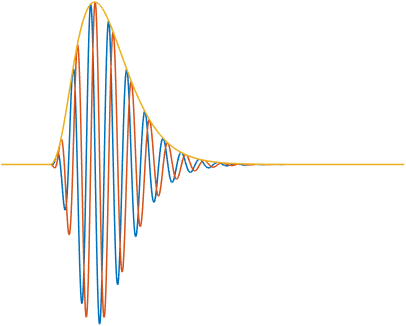
\includegraphics[height=2cm,width=3.5cm]{gammatone_Q4.png}}
 \put(2.5,0.0){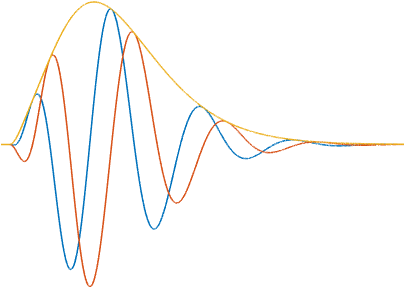
\includegraphics[height=2cm,width=3.5cm]{gammatone_Q1.png}}
\end{picture}
\caption{
\label{fig:gammatones}
Left: Gammatone wavelet $\boldsymbol{\psi_{\gamma_1}}(t)$ with a quality factor of $Q=4$.
Right: Gammatone wavelet $\boldsymbol{\psi_{\gamma_2}}(t)$ with a quality factor of $Q=1$.
Blue and red oscillations represent the real and imaginary parts. The orange envelope represents
the complex modulus.}
\end{center}
\end{figure}

We define a wavelet filter bank $\{\psi_\lambda\}_{\lambda>0}$ by dilating a mother wavelet $\psi$ according to
\begin{equation}
	\psi_\lambda(t) = \lambda \psi(\lambda t).
\end{equation}
The mother wavelet $\psi$ is assumed to be analytic, that is with a zero Fourier transform for negative frequencies. In addition, we will the Fourier transform of $\psi$ to be centered around $1$. Consequently, $\psi_\lambda$ is centered at the frequency $\lambda$. A function $\psi$ that fulfills these criteria is the analytic gamma wavelet, illustrated in Figure \ref{fig:gammatones}. Its form is given explicitly by
\begin{equation}
	\psi(t) = ???
\end{equation}
We shall have use for wavelets of different quality factors $Q$. To begin with, we shall take $Q = 4$.

Given a signal $x$, we decompose it using the wavelet filter bank to obtain
\begin{equation}
	x \ast \psi_\lau(t) \quad \mathrm{for~}\lau>0,
\end{equation}
known as the wavelet decomposition of $x$. The dilation structure of the wavelet filter bank means that we do not need to sample $\lau$ continuously. Rather, it is sufficient to sample $\lau$ as $2^{j/Q}$, where $Q$ is the quality factor of the mother wavelet $\psi$. This means that we sample uniformly in log-frequency $\log \lau$.

The wavelet decomposition itself is very sensitive to time-shifting and time-warping, which can be reduced by taking the complex modulus. The result is known as the wavelet scalogram and we denote it by
\begin{equation}
	x_1(t, \log \lau) = | x \ast \psi_\lau(t) |.
\end{equation}
A sample scalogram is given in Figure \ref{fig:scalogram}.

The scalogram provides a useful representation of the time-frequency content of a signal. At a given point $(t, \log \lau)$, it gives the intensity of $x$ at time $t$ and log-frequency $\log \lau_1$. However, it does not have the desired invariance and stability properties. To achieve this, we average the scalogram in time using a lowpass filter $\phi_T(t)$ of duration $T$ to give
\begin{align}
	\nonumber
	S_1 x(t, \log \lau) &= x_1(\cdot, \log \lau) \ast \phi_T(t) \\
	&= | x \ast \psi_\lau | \ast \phi_T(t).
\end{align}
In our configuration $\phi_T$ is given by a Gabor filter centered at frequency $0$ with the desired bandwidth $T$ in time. The coefficients $S_1 x$ are known as first-order time scattering coefficients and are comparable to the commonly used mel-frequency spectrogram coefficients \cite{davis-mermelstein}.

The averaging by $\phi_T$ loses fine-scale structre in the scalogram $x_1$. To recover this, we calculate a second wavelet decomposition, this on the scalogram, along the time axis. Instead of the quality factor $Q = 4$ used in the first decomposition, we now use $Q = 1$. As before, we compute the complex modulus and obtain
\begin{align}
	\nonumber
	x_2(t, \log \lau, \log \lad) &= x_1(\cdot, \log \lau) \ast \psi_\lad(t) \\
	&= |\,| x \ast \psi_\lau | \ast \psi_\lad (t) |.
\end{align}
This second-order wavelet scalogram describes the modulation structure of the frequency band centered at $\log \lau$ of the first-order scalogram $x_1$. It is therefore closely related to modulation spectrograms \cite{atlas}, but are defined using wavelet decompositions instead of short-time Fourier transforms.

Again, to obtain invariance, the second-order scalogram $x_2$ is averaged in time using the lowpass filter $\phi_T$ to give
\begin{align}
	\nonumber
	S_2 x(t, \log \lau, \log \lad) &= x_2(\cdot, \log \lau, \log \lad) \\
	&= |\,| x \ast \psi_\lau | \ast \psi_\lad | \ast \phi_T(t),
\end{align}
which are known as second-order time scattering coefficients. Like modulation spectrograms, these coefficients provide information on the modulation structure of the signal $x$ at log-frequency $\log \lau$, but does so in a stable manner due to the wavelet construction. In this way, they are more closely related to constant-Q averaged modulation spectrograms \cite{ellis-mcdermott}. We note that the above procedure can be continued for third- and higher-order scattering coefficients, but that for most applications, first- and second-order coefficients suffice.

Concatenating all the first-order scattering coefficients into one vector
\begin{equation}
	S_1x(t) = \{S_1x(t, \log \lau)\}_{\lau>0},
\end{equation}
and doing the same for the second-order coefficients
\begin{equation}
	S_2x(t) = \{S_2x(t, \log \lau, \log \lad\}_{\lau>0, \lad>0},
\end{equation}
we can combine all of them into one scattering vector at time $t$
\begin{equation}
	Sx(t) = \{S_1x(t), S_2x(t)\}.
\end{equation}
It is important here to remark that, although the above formulas cover continuous domains in $t$, $\log \lau$, and $\log \lad$, these variables can all be sampled discretely without great loss of information. As mentioned earlier, $\log \lau$ and $\log \lad$ can be sampled uniformly with a step proportional to $1/Q$. In addition, the lowpass nature of the scalogram $x_1$ in time ensures that many coefficients in $x_2$ will be negligible for large values of $\log \lad$. As a result, these can be safely excluded from the transform. Finally, the lowpass filtering by $\phi_T$ ensures that we can sample the final scattering vector $Sx$ along multiples of $T$ in time.

\section{Data augmentation}

\section{Discussion}

\begin{table}[!htbp]
\centering
\caption{
Cross-validation results.
\label{table:single-label-durations}}
\begin{tabular}{llll}
\toprule
Scene & Baseline & Temporal scattering & Temporal scattering \\
           &               &  (1 azimuth)  & (5 azimuths) \\
 \midrule
beach & 72.0 $\pm$ 19.0 & & 84.9 $\pm$ 11.7 \\

bus & 62.0 $\pm$ 19.6 & & 91.3 $\pm$ 14.4 \\

cafe/restaurant & 83.9 $\pm$ 12.1 & & 57.1 $\pm$ 20.5 \\

car & 75.7 $\pm$ 17.7 & & 93.7 $\pm$  \phantom{0}6.3 \\

city center & 85.6 $\pm$ 18.5 & & 92.8 $\pm$  \phantom{0}8.9 \\

forest path & 65.9 $\pm$ 26.5 & & 96.4 $\pm$  \phantom{0}7.2 \\

grocery store & 76.6 $\pm$ 22.3 & & 84.3 $\pm$ 15.6 \\

home & 79.5 $\pm$ 18.6 & & 64.2 $\pm$ 26.3 \\

library & 61.3 $\pm$ 30.5 & & 81.1 $\pm$  \phantom{0}7.5 \\

metro station & 85.3 $\pm$ 18.0 & & 98.7 $\pm$  \phantom{0}2.7 \\

office & 91.1 $\pm$ \phantom{0}7.9 & & 86.1 $\pm$ 27.8 \\

park & 24.5 $\pm$ 15.6 & & 75.6 $\pm$ 10.5 \\

residential area & 75.4 $\pm$ 29.1 & & 55.8 $\pm$ 20.2 \\

train & 36.7 $\pm$ 10.8 & & 57.1 $\pm$ 15.3 \\

tram & 89.5 $\pm$ 17.5& & 86.4 $\pm$ 11.7 \\

\bottomrule

average & 71.3 $\pm$  \phantom{0}3.8 & & 80.4 $\pm$  \phantom{0}3.5
\end{tabular}
\end{table}

\section{Conclusion}
This technical report presents 

\bibliography{Lostanlen_DCASE2016}

\end{document}


